\documentclass{article}
\usepackage{graphicx}
\graphicspath{ {images/} }


\begin{document}
\title{Python DIC Documentation}
\author{Charlie Bourigault\\ bourigault.charlie@gmail.com}
\date{September 2016}
\maketitle
\thispagestyle{empty}
\begin{abstract}
  This document constitutes a detailed guide of the Python digital image correlation software from Fraunhofer IWM. Fonctions and capabilities of the software are presented along with various example to help you familiarize with the application. For any other information or any comment on the software please contact the author or visit the GitHub repository (Python\_DIC) on https://github.com/.

\end{abstract}
\newpage
\tableofcontents


\newpage
\section*{Introduction}
\addcontentsline{toc}{section}{Introduction}
\label{sec:Introduction}
\vspace{.5cm}
\indent\indent Digital Image Correlation (or DIC) is used in several domains and mainly in engineering and sciences. It employs different techniques to track markers placed on images and provides accurate measurement results of changes in those images. Users can acquire displacements, strains fields along with other information in a simplified manner.\\
\newline
\indent The PythonDIC software comes with a variety of functions and algorithms to accompany you through the process of image correlation. This documentation offers an overview of the software capabilities.\\
\newline\indent Software updates are released regularly and this documentation may not be fully comprehensive with upcoming functions. Please visit the github project (Python\_DIC) to get last updates information.


%%%%%%
\newpage
\section{Installation Instructions}
\label{sec:Installation Instructions}
\vspace{.5cm}
\indent\indent The Python\_DIC application is cross-platform and have been tested on Window 7, MacOS (10.11) and Linux (Ubuntu 16.4). It runs on Python 3.x and requires the installation of some external packages. We recommend you to stick with the following installation procedure to avoid any malfunction or unintended crashes of the software.\\
\newline Required Packages:
\begin{itemize}
  \item matplotlib
  \item scipy
  \item opencv3
\end{itemize}
\newline
Miniconda3 is used to manage and simplify the Python installation process.


\subsection{Windows Systems}
\label{sub:Windows Systems}
  \subsubsection{Download and Install Miniconda3}
\label{subs:Download and Install Miniconda3}
\indent\indent In order to run Python on your computer, a Python environment needs to be installed. Using a package manager as Miniconda (a light version of Anaconda) simplify the process and provides a good management tool for external libraries.\\
\newline
\indent Visit \textit{\href{http://conda.pydata.org/miniconda.html}} and download the last Miniconda \underline{3} (Python 3.x 64 bits) package for Windows. Follow then the installation instructions.
\subsubsection{Install Required Libraries}
\label{subs:Install Required Libraries}
\indent\indent Several libraries are compulsory for the Python DIC software to run properly. The installation process using the Miniconda environment is simplified and convenient. Here is how it works.
\begin{itemize}
  \item Open the Command Window (\texit{Start \textgreater \space Search \textgreater \space cmd})
  \item Type in : \textit{conda install matplotlib}
  \item Follow the instruction to install the package
  \item Do the same with the \textit{scipy} and \textit{pandas} libraries
\end{itemize}
\newline
\indent\indent OpenCV3 is a library which also needs to be installed. The release available on the default conda channel is not compatible with the latest Python3.x version when I'm writing these lines. However, the correct version of OpenCV have been compiled by different people and is available on different channels.\\
\newline
\indent The OpenCV3 compiled version for Windows systems is available on the \textit{menpo} channel. Here is how to install it.
\begin{itemize}
  \item Terminal Command : \textit{conda install -c menpo opencv3}
\end{itemize}
\newline
\indent\indent In case the package is not available on this channel, use \textit{anaconda search opencv3} to find another place to download it from. (You may need the anaconda client to search for libraries. To install it, use \textit{conda install anaconda-client}).\\
\newline
\indent Libraries have been installed. The software is ready to be started.
\subsubsection{Start Python DIC}
\label{subs:Start Python DIC}
  \indent\indent Once the Python DIC files have been download from the GitHub repository (and extracted if needed). Follow these simple steps.
  \begin{itemize}
    \item Navigate to the folder where the Python DIC files have been extracted.
    \item Right-click on DIC.py and select \textit{Open With..}
    \item Select \textit{Browse}
    \item Navigate to your Miniconda folder (Default: \textit{C:/Users/\textless SessionName\textgreater /Miniconda3})
    \item Chose \textit{pythonw.exe} as a default program.
  \end{itemize}
  \newline
  \indent\indent The program can also be started using the windows Command Line. Navigate to the Python DIC folder with the \textit{cd} command and start the Python DIC program using : \textit{python DIC.py}.\\
  \newline


\subsection{Unix Systems}
\label{sub:Unix Systems}
  \subsubsection{Download and Install Miniconda3}
\label{subs:Download and Install Miniconda3}
  \indent\indent In order to run Python on your computer, a Python environment needs to be installed. Using a package manager as Miniconda (a light version of Anaconda) simplify the process and provides a good management tool for external libraries.\\
  \newline
  \indent Visit \textit{\href{http://conda.pydata.org/miniconda.html}} and download the last Miniconda \underline{3} (Python 3.x 64 bits) package for your system. Follow then the installation instructions.
\subsubsection{Install Required Libraries}
\label{subs:Install Required Libraries}
  \indent\indent Several libraries are compulsory for the Python DIC software to run properly. The installation process using the Miniconda environment is simplified and convenient. Here is how it works.
  \begin{itemize}
    \item Open a Terminal window
    \item Type in : \textit{conda install matplotlib}
    \item Follow the instruction to install the package
    \item Do the same with the \textit{scipy} library
  \end{itemize}
  \newline
  \indent\indent OpenCV3 is a library which also needs to be installed. The release available on the default conda channel is not compatible with the latest Python3.x version when I'm writing these lines. However, the correct version of OpenCV have been compiled by different people and is available on different channels.\\
  \newline
  \indent The OpenCV3 compiled version for Unix systems is available on the \textit{menpo} channel. Here is how to install it.
  \begin{itemize}
    \item Terminal Command : \textit{conda install -c menpo opencv3}
  \end{itemize}
  \newline
  \indent\indent In case the package is not available on this channel, use \textit{anaconda search opencv3} to find another place to download it from. (You may need the anaconda client to search for libraries. To install it, use \textit{conda install anaconda-client}).\\
  \newline
  \indent Libraries have been installed. The software is ready to be started.
\subsubsection{Start Python DIC}
\label{subs:Start Python DIC}
  \indent\indent Once the Python DIC files have been download from the GitHub repository (and extracted if needed). Follow these simple steps.
  \begin{itemize}
    \item Open a Terminal window
    \item Navigate to the folder containing the Python DIC \textit{.py} files (use the \textit{cd} command)
    \item Type in : \textit{python DIC.py}
  \end{itemize}


%%%%%%
\newpage
\section{Interface}
\label{sec:Interface}
\vspace{.5cm}
  \indent\indent On startup, the Python DIC application proposes two options. One can either start a new correlation process or open a previously made analysis to access results and enhance the data if necessary.


  \subsection{New Analysis}
  \label{sub:New Analysis}
    \indent\indent When starting a new analysis, the software asks for an image to start with. Images from the same type present in the folder will be automatically selected and listed. Unselect images which shouldn't be part of the analysis, give your analysis a name and the grid creation tool will start.\\

\begin{figure}[!h]
   \centering
   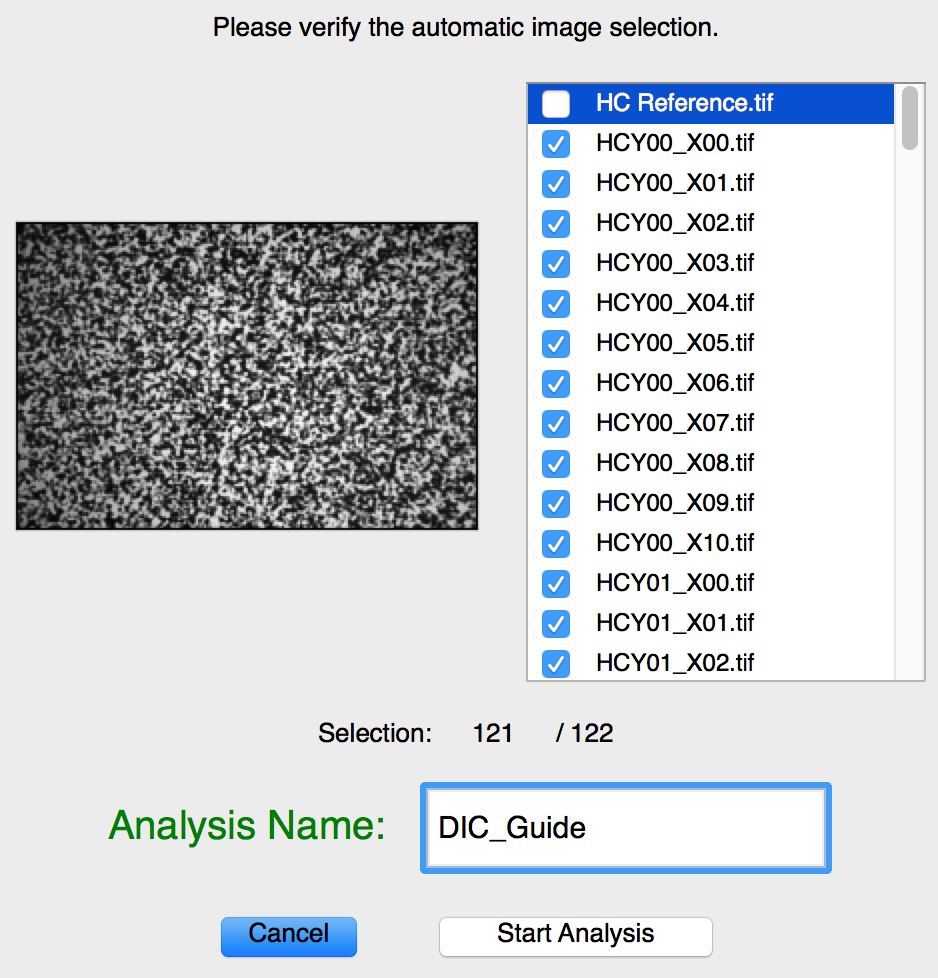
\includegraphics[scale=.4]{image_selection}
   \caption{New Analysis: Image Selection}
\end{figure}

\newline
\indent\indent The grid creation tool is divided into three main areas. The top part provides tools to build a grid necessary for the correlation process. Under this tools zone, the application is separated in two entities : the left side displays your images and the grid, the right side takes care of filters for your images.\\
\newpage


    \subsubsection{Grid tools and information}
    \label{subs:Grid Tools and Information}
      \indent\indent The top part of the grid creation tool offers different means to create a grid for your analysis. It also displays information and parameters which will be used in the correlation process.

\begin{figure}[!h]
   \centering
   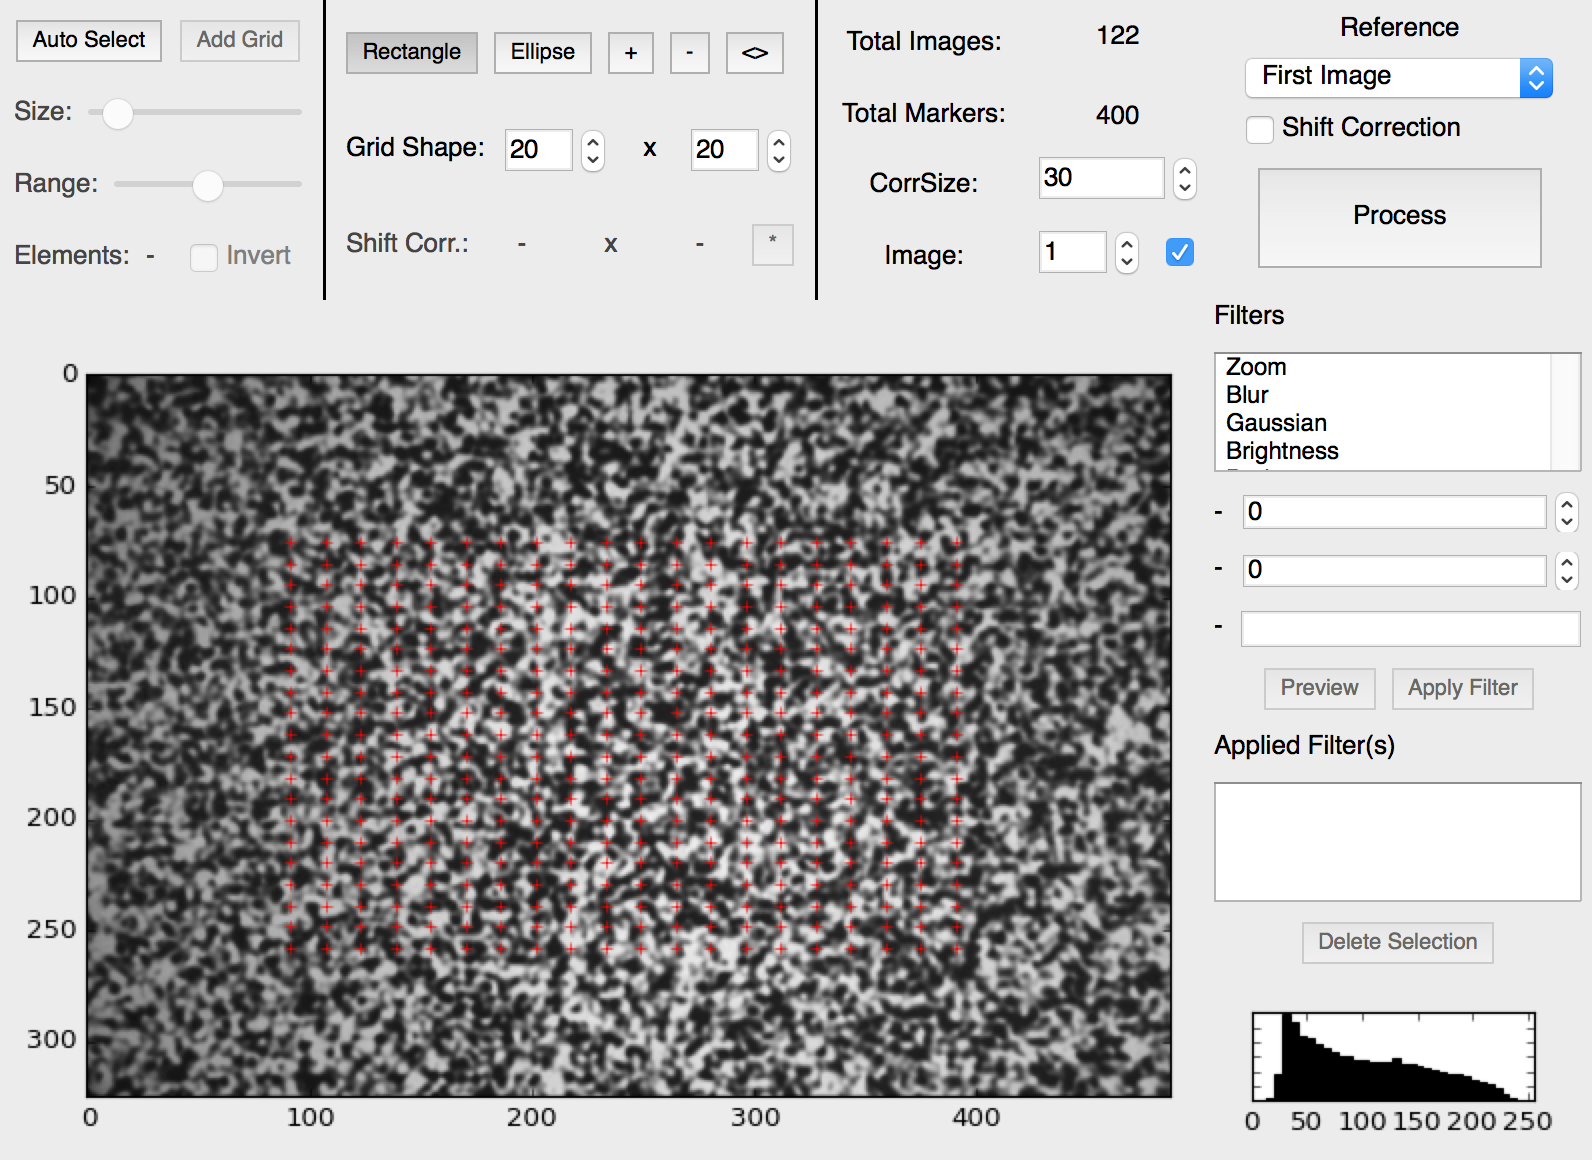
\includegraphics[scale=.4]{grid_creation}
   \caption{New Analysis: Grid Definition}
\end{figure}

\paragraph{Grid Creation\\\newline}
\label{par:Grid Creation}
\indent In order to run an analysis, a grid have to be defined. A grid is a set of markers with different coordinates which constitute the base of the correlation. When the images will be processed, the algorithm will track each marker on each image to determine the local displacement inside of your set of images.\\
\newline
There are three types of grid available:
\begin{itemize}
  \item \textit{Rectangular} : The grid shape parameters defines the number of marker in X and Y direction
  \item \textit{Ellipsoidal} : The grid shape parameters defines the number of marker in X and Y direction and an ellipsoidal mask is applied
  \item \textit{Single Marker (+)} : A 1x1 grid with only one marker
\end{itemize}
\newline
\indent\indent To create a grid, select one of the tool above, click and drag your mouse on the image at the position where you want to draw your grid.\\
\newline
\indent The \textit{(-)} tool can be used to remove one or several markers. Click and drag your mouse on the area where you want to delete markers.\\
\newline
\indent A grid can be moved by using the \textit{(\textless\textgreater)} tool. Click on the grid you want to move and drag it on the new location.\\
\newline\newline
\indent One or several grids can be defined. They will be saved as different entities and can later be evaluated independantly from each other.

\paragraph{Parameters\\\newline}
\label{par:Parameters}
\newline
\indent\indent Different information are available before starting the correlation process. The number of images along with the number of markers created are displayed for your information. You can use the image input box to navigate through your images and individually remove some of these by unchecking the box on the right. A corrsize has to be defined to run the analysis.\\
\newline
\indent The corrsize represent the size in pixel of the squared zone in which each marker will be tracked. If the corrsize is too small, the algorithm may not be able to track markers properly as they may go out of the range. However, a high corrsize value will result in high computation time. We recommend using values between 20 and 30 pixels for small displacements which gives fast and accurate results.\\
\newline
Three modes are available to evaluate the markers displacement:
\begin{itemize}
  \item \textit{First Image Reference}: The first image will be used has a reference for each image. This is the recommended mode, which gives the most accurate results. However, if displacements on an images are greater than the corrsize value, the algorithm may not be able to track markers.
  \item \textit{Previous Image Reference}: For each image, the reference markers to track will be the previously tracked markers (ie: the base grid is redefined for each images to the new marker positions). This method reduce the chance of lost markers during the process. However, the displacement error is increased with the time and results can get inaccurate after a certain amount of images.
  \item \textit{Shifted Image Reference}:  The reference image is defined with a step. The first image will be the reference until this step is reached, then, the base grid will be redefined to the current image minus the step. This method can be used if you have big displacements after a certain number of images. You'll get accurate results for the beginning of the analysis and still keep trace of markers for the rest of images which a slighly reduced accuracy.
\end{itemize}


    \newpage
    \subsubsection{Shift correction, filters and file importation}
    \label{subs:Shift Correction and Filters}

    \vspace{.3cm}
      \paragraph{Shift Correction\\\newline}
      \label{par:Shift Correction}
        \newline
\indent\indent The shift correction have been introduced in the Python DIC application to face problems such as camera lateral moves. In order to reduce the amount of pixel displacements due to the camera moves, a first general image correlation is performed without markers in order to align images. Once the alignment is performed, a normal marker correlation can be performed.\\
\newline
\indent The use of the shift correction may affect the accuracy of your results. It may lead to wrong marker displacement calculation and is therefore non recommended, although it can be used in extrem cases.\\
\newline
The shift correction is performed prior to the correlation process. The procedure to use is the following:
\begin{itemize}
  \item Check the shift correction option
  \item Select a relatively large area (if possible outside of the grid location) by clicking and draging your mouse on the image
  \item Click on the \textit{Track} button and wait until the end of the process
  \item Click on the \textit{Confirm} button to validate
\end{itemize}
\newline
\indent\indent At the end of the process, the shift correction values are available for each image. Use the input text box displaying the image number to navigate in the image and review the shift correction value. You can modify these values in case of wrong recognition by clicking on the \textit{*} button next to the shift values.\\
\newline
\indent Uncheck the shift correction tool to cancel the procedure or to change the tracking area. Shift corrections values will be taken in account once the grid is created and the correlation process started.


      \paragraph{Images Filters\\\newline}
      \label{par:Images Filters}
        \newline
\indent\indent Different filters can be applied to your set of images before any analysis. These filters allow you to improve the quality of the correlation by performing operations on your images such as contrast enhancement or noise reduction.\\
\newline
\indent The Python DIC software will \textbf{not} modify any of your images. Filters are applied after the reading process and do \textbf{not} affect the original files.\\
\newline
Filters are simple and convenient to use:
\begin{itemize}
  \item Select one of the available filters
  \item Modify parameters specific to the selected filter
  \item Click on the \textit{Preview} button to have a instant view of the filter effect
  \item Click the \textit{Apply Filter} button when you're satisfied to add the filter to applied filters list
  \item Select any filter in the applied filter list and click the \textit{Delete Selection} button to remove the filter from the applied filters list
\end{itemize}
\newline
\indent \textit{Note}: An histogram is available and provides an instant view of the gray scale dispersion on the current image.


      \paragraph{Grid and Filters Importation\\\newline}
      \label{par:Grid and Filters Importation}
        \newline
\indent\indent An option have been included to import grids and filters from previously performed analysis. Under the \textit{File} menu, you will find the \textit{Open Grid} and \textit{Open Filter} options.\\
\newline
\indent Select the project folder containing the grid(s) and/or the filter(s) that you want to import in your analysis. The software will then look for the grid files or the filter file in this folder and use the same parameters for the current analysis.


  \newpage
  \subsection{Data Analysis - Visualisation}
  \label{sub:Data Analysis - Visualisation}
  \vspace{.3cm}
    \indent\indent The visualisation tool is automatically opened after a correlation process. It is also accessible on the start-up widget by clicking on the \textit{Open Analysis} button.\\
\newline
There is two type of element in the visualisation window:
\begin{itemize}
  \item A certain amount of plots
  \item A control area with information
\end{itemize}
\newline
The control area is fixed and displays information on the analysis and the current image selected.\\
You can navigate through the data using the two cursor available in the control area.\\

\begin{figure}[!h]
   \centering
   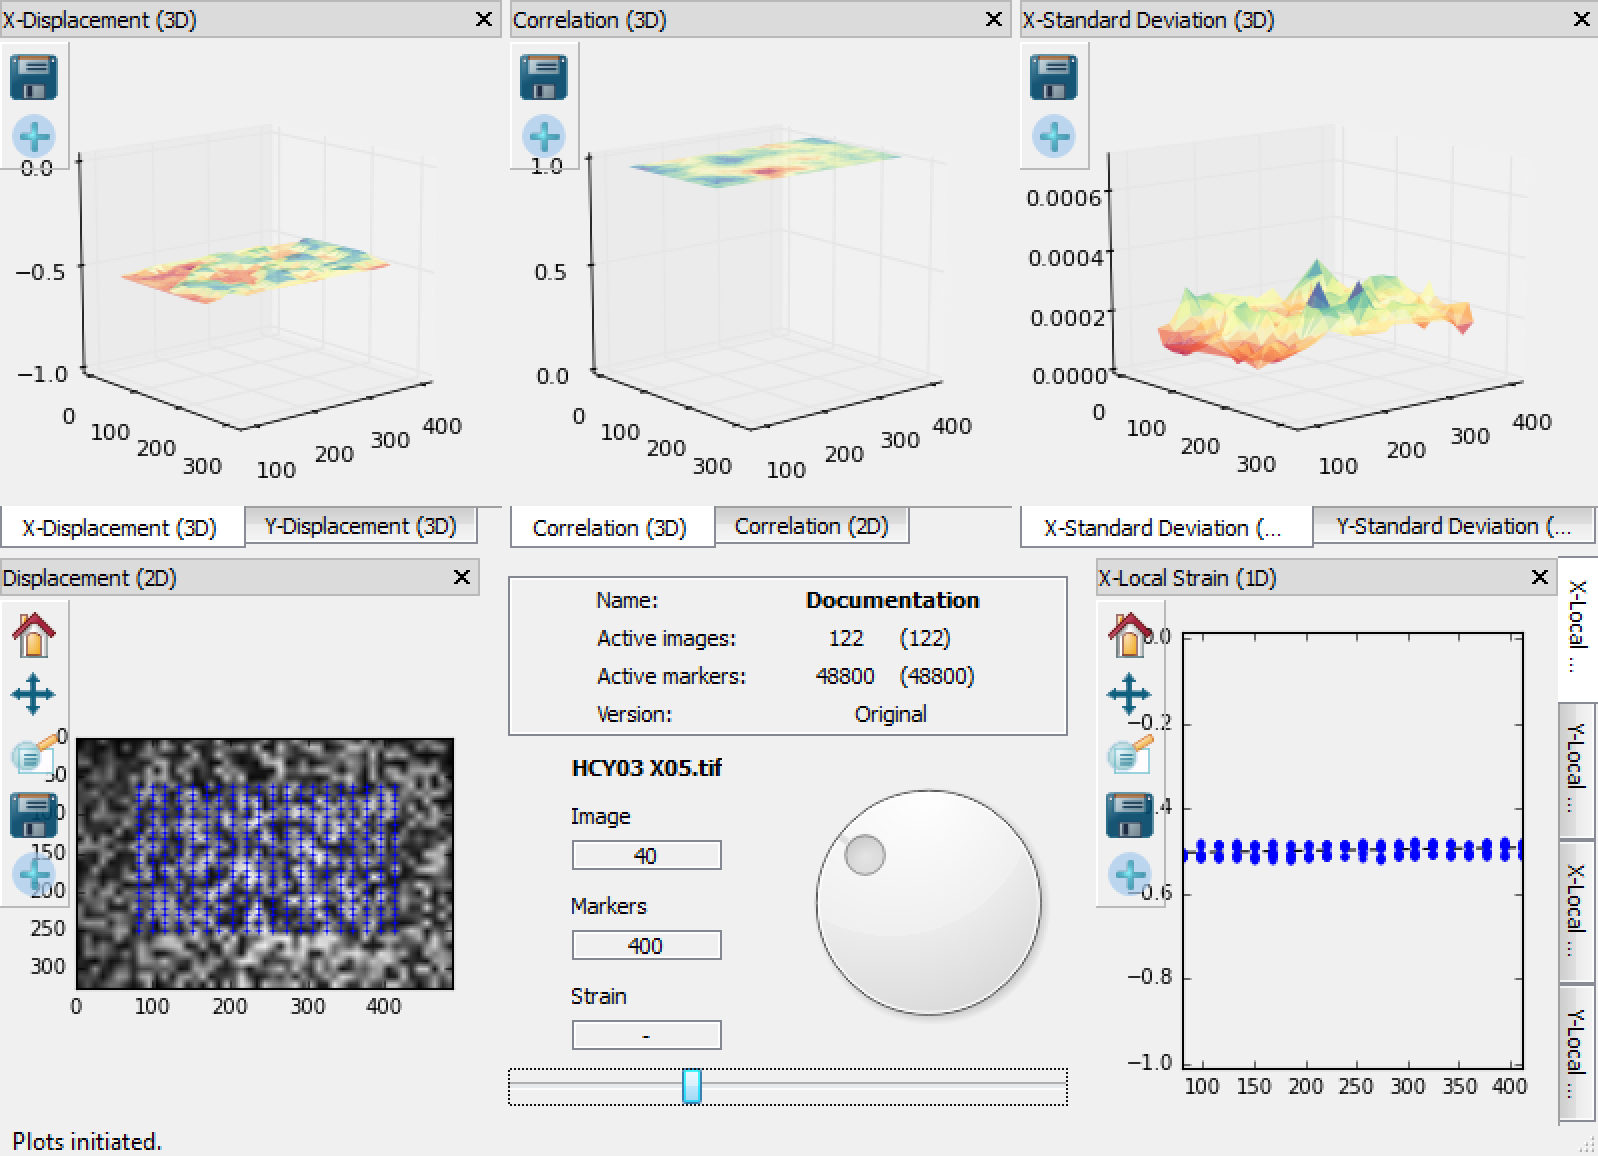
\includegraphics[scale=.4]{visualisation}
   \caption{Visualisation : Navigation through results}
\end{figure}

\newline
\noindent Plots are located around the control area and can be re-organized by the user.
\begin{itemize}
  \item Click and drag a plot to move it
  \item Close unwanted plots using the individual cross
  \item Open plots by right-clicking on an empty area or next to the menu
\end{itemize}
\newline
When the data is refreshed, only the visible opened plots are taken in account. For large analysis, closing unnecessary plots will sensibly decrease the refreshing time.\\
You can also stack plots on top of each other for a quick access. This will not affect the refreshing time as only visible plots are reloaded.\\
\newline
For each single plot, you can use the toolbar to save the plot as an image and zoom/pan on your data. Different display options are also available, click on the \textit{+} button in the toolbar to get access to parameters.
\vspace{.5cm}
\begin{figure}[!h]
   \centering
   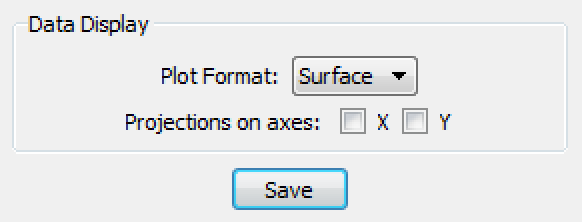
\includegraphics[scale=.8]{plot_options}
   \caption{Visualisation : 3D plots options}
\end{figure}


\newpage
\section{Cleaning Procedures and Options}
\label{sec:Cleaning Procedures and Options}
\vspace{.5cm}

  \subsection{Grid Management}
  \label{sub:Grid Management}
    \vspace{.2cm}
    \indent\indent You can perform separate grid calculation on a single analysis. To do so, draw several grids before starting a correlation in the grid creation tool. Once the calculation done, you'll be able to analyze these grid separately.\\
\newline
\indent If several grids have been created, they'll be dissociated in the visualisation tool. You are then able to differentiate the strain in one grid compared to another. Using the instance management tool, you can temporaly hide one or several grids to focus on the one (or those) that you're interested in.
\begin{itemize}
  \item Go into \textit{Masks \textgreater Manage Grids}
  \item Chose the grids you want to hide/display
  \item Validate to apply changes
\end{itemize}
\newline

\begin{figure}[!h]
   \centering
   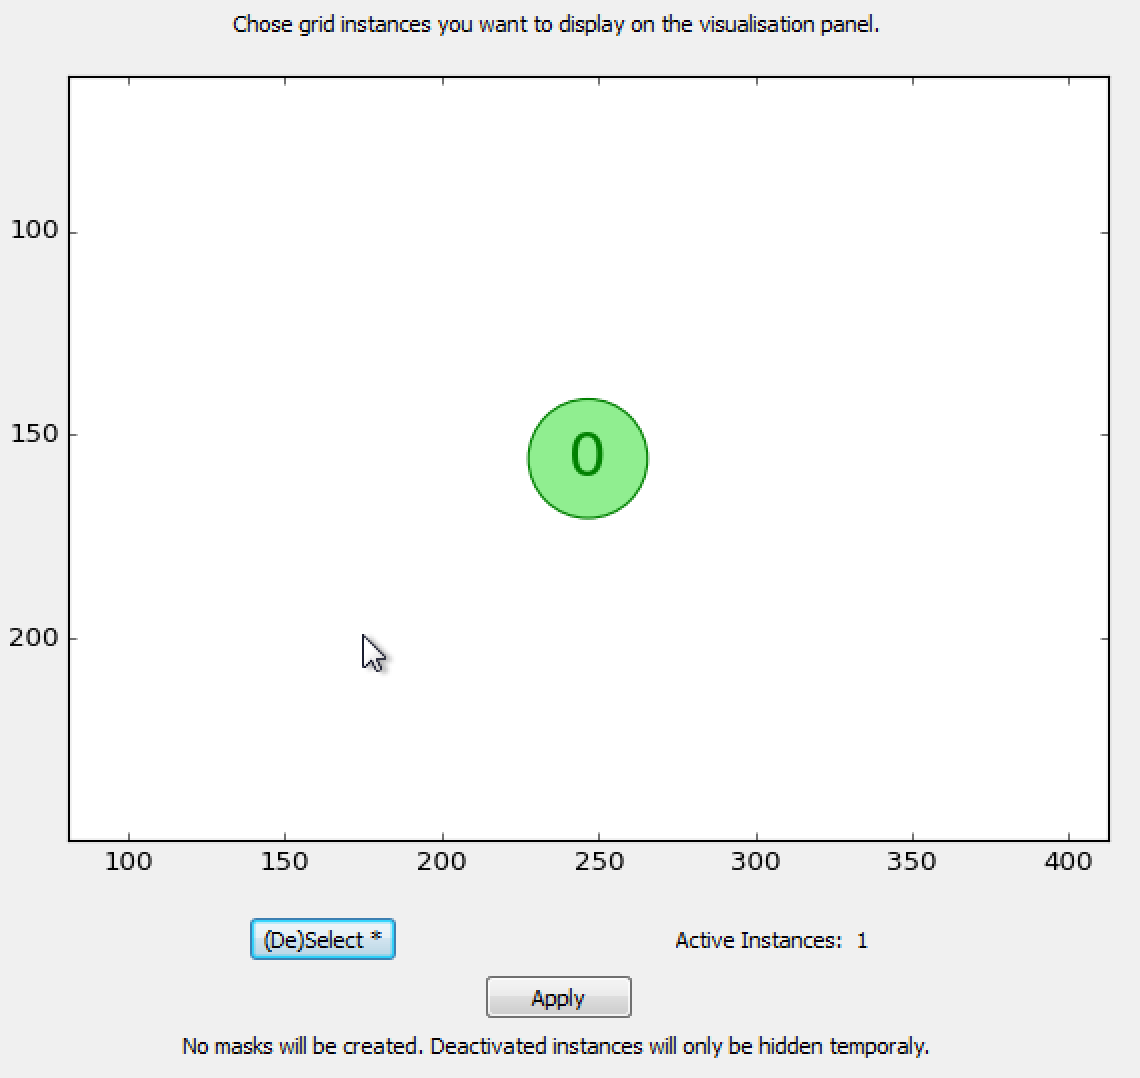
\includegraphics[scale=.4]{grid_management}
   \caption{Grid Management - Active instances displayed in green}
\end{figure}

When you hide or display grid instances, the changes made are not saved and all the grid will be displayed by default on the next start-up.


  \newpage
  \subsection{Mask Images}
  \label{sub:Mask Images}
    \vspace{.2cm}
    \indent\indent In the \textit{Masks} menu, you'll find the \textit{Mask Images} feature. This option provides an easy way to remove images from your analysis. Select the images that you want to mask in your analysis to hide them from the analysis.\\

\begin{figure}[!h]
   \centering
   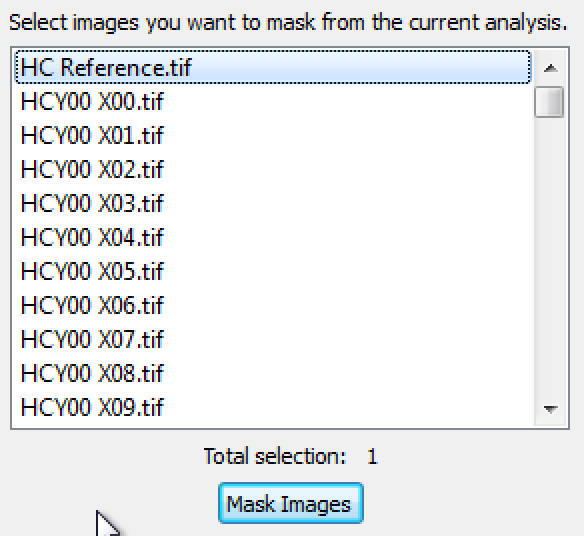
\includegraphics[scale=.6]{mask_images}
   \caption{Mask Images - Select images to hide}
\end{figure}

\newline
\indent When a mask is applied, the previous state of the analysis is automatically saved in the analysis folder.\\
On start-up, the software will load the last mask version by default. If you made a mistake or want to bring back your data, you can open a previous version by using the \text{Open Mask/Version} option in the \textit{File} menu.\\
\newline
\indent Please keep in mind that when a mask is applied, the data is only hidden and not modified. An older version can always be loaded.


  \newpage
  \subsection{Mask Markers}
  \label{sub:Mask Markers}
    \vspace{.2cm}
    \indent\indent Using the \textit{Mask Markers} feature will allow you to manually select badly correlated data in order to hide it from you analysis. Select the markers that do not behave as expected and apply the mask to enhance the analysis results.\\

\begin{figure}[!h]
   \centering
   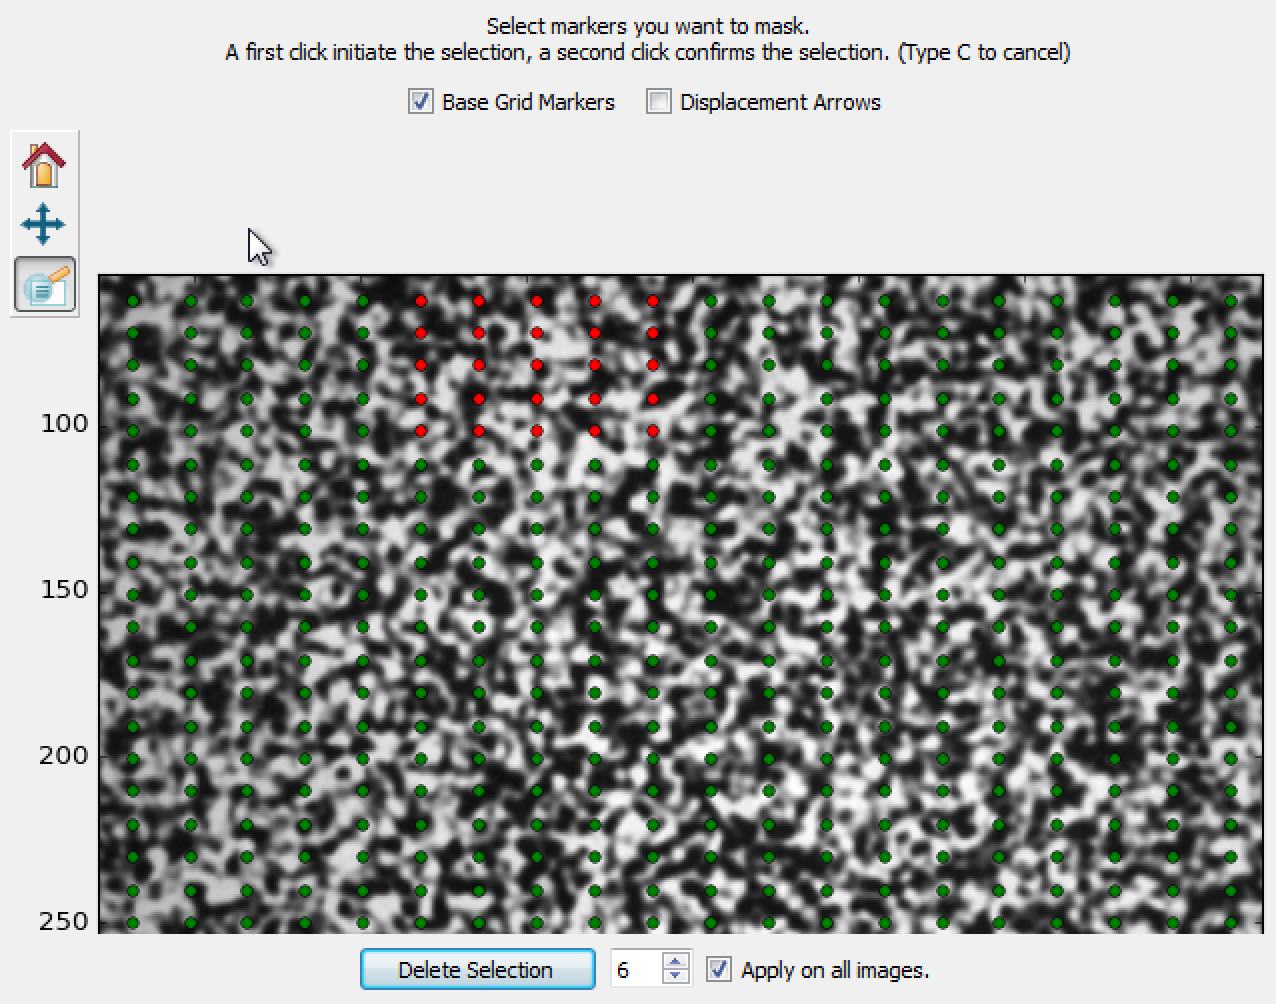
\includegraphics[scale=.4]{mask_markers}
   \caption{Mask Markers - Hide manually selected markers}
\end{figure}

\newline
\indent When a mask is applied, the previous state of the analysis is automatically saved in the analysis folder.\\
On start-up, the software will load the last mask version by default. If you made a mistake or want to bring back your data, you can open a previous version by using the \text{Open Mask/Version} option in the \textit{File} menu.\\
\newline
\indent Please keep in mind that when a mask is applied, the data is only hidden and not modified. An older version can always be loaded.


  \newpage
  \subsection{Displacement versus position}
  \label{sub:Displacement versus position}
    \vspace{.2cm}
    \indent\indent The \textit{Disp. vs Pos.} feature from the \textit{Masks} menu helps you to compare the displacement of each marker depending on its position in the X or Y direction. Select the markers that you would like to hide and confirm to apply the mask on your data.\\
\newline
\indent This tool gives you a fast and easy way to detect wrong behaviour in your markers. All markers will in most of the case follow a certain trend in one direction and you can then locate markers with correlation issues.\\

\begin{figure}[!h]
   \centering
   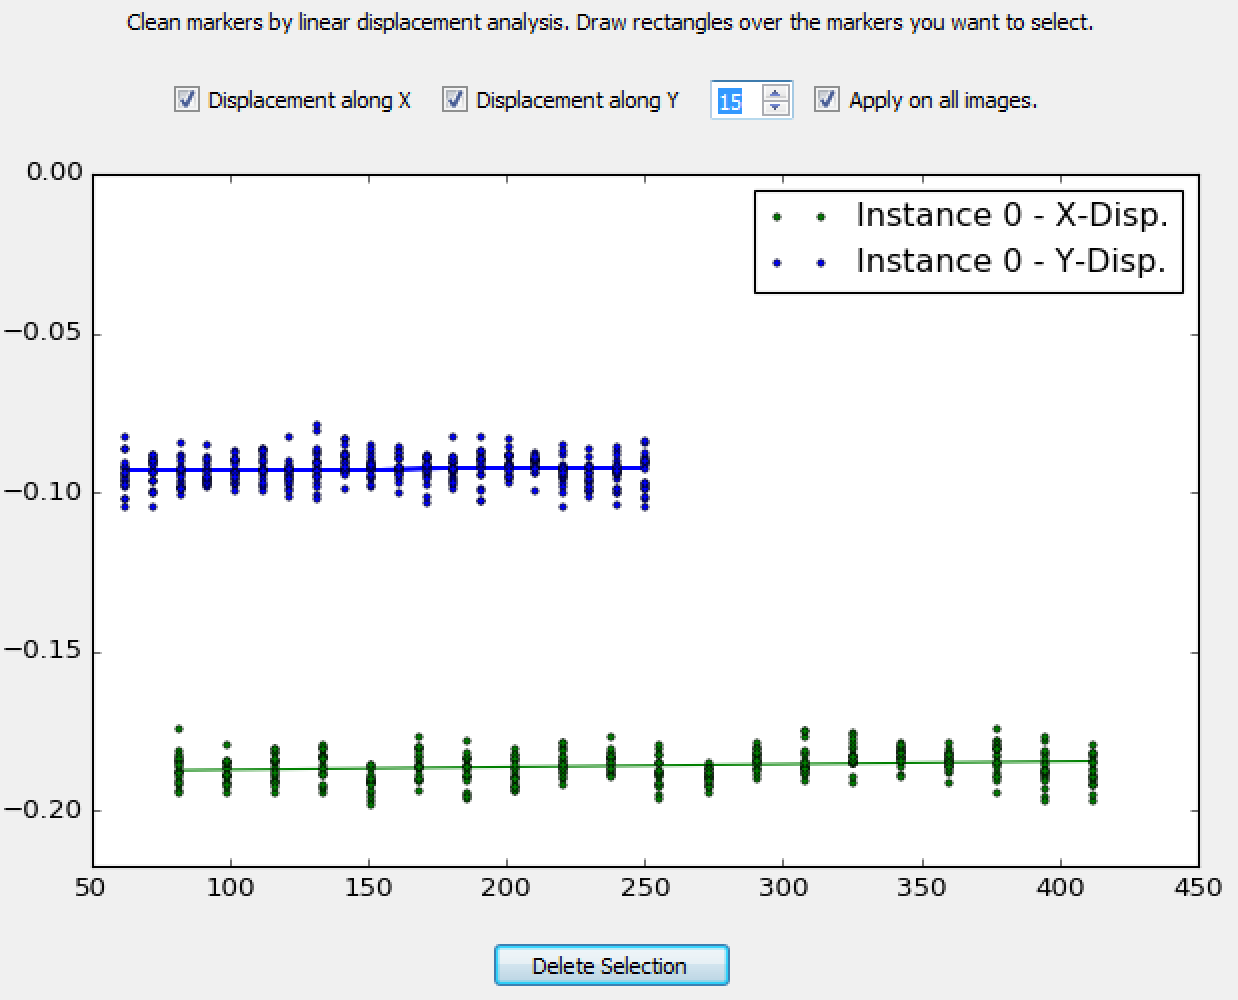
\includegraphics[scale=.4]{disp_vs_pos}
   \caption{Disp. vs Pos. - Hide markers with wrong behaviour}
\end{figure}

\newline
\indent When a mask is applied, the previous state of the analysis is automatically saved in the analysis folder.\\
On start-up, the software will load the last mask version by default. If you made a mistake or want to bring back your data, you can open a previous version by using the \text{Open Mask/Version} option in the \textit{File} menu.\\
\newline
\indent Please keep in mind that when a mask is applied, the data is only hidden and not modified. An older version can always be loaded.


  \newpage
  \subsection{Relative neighbors displacement}
  \label{subs:Relative neighbors displacement}
    \vspace{.2cm}
    \indent\indent The \textit{Relative neighbors disp.} tool offers you a powerful way to automatically clean your data.\\
\newline
\indent The algorithm will provide you a graph displaying the relative displacement of each marker compared to his closest neighbors during the whole correlation process. A marker with high displacements compared to its neighbors may be badly correlated and should be masked. You can also detect when a marker starts to behave differently compared to its neighbors.\\
\indent In order to masked the unwanted markers, move the two upper and lower red lines on the graph representing the maximum relative displacement for each marker. If a marker cross the upper or lower limit, it'll automatically be masked.\\

\begin{figure}[!h]
   \centering
   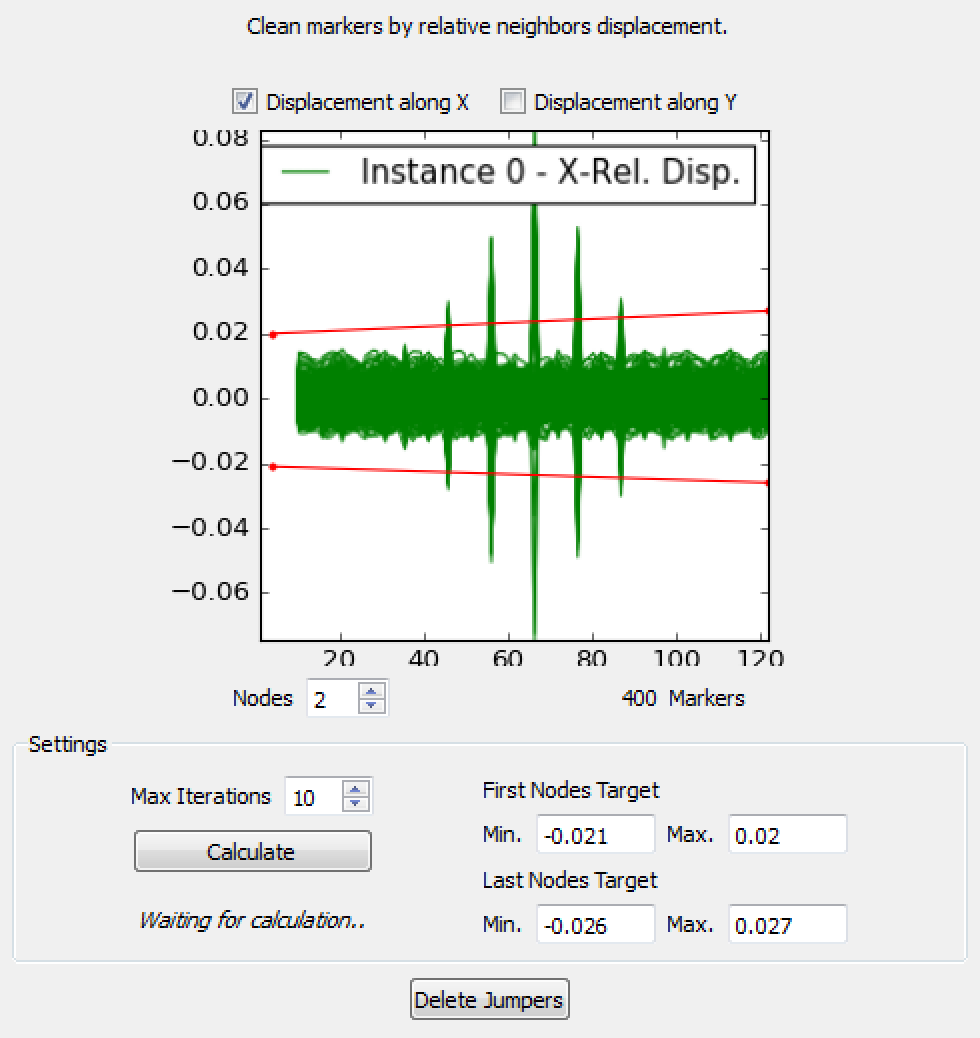
\includegraphics[scale=.6]{relative_neighbors}
   \caption{Relative Neighbors Disp. - Define upper and lower limits}
\end{figure}

\newpage
\indent A masked marker may generate new high relative displacement in the new neighborhood of some markers. The algorithm will automatically recalculate the relative displacement after a deletion and continue the cleaning if some markers are then crossing the predefined upper and lower limits. Once all the unwanted have been masked (or the iteration number is reached), the new graph is displayed and you can then confirm the calculation to apply the mask to your data or set new limits.\\
\newline
\indent When a mask is applied, the previous state of the analysis is automatically saved in the analysis folder.\\
On start-up, the software will load the last mask version by default. If you made a mistake or want to bring back your data, you can open a previous version by using the \text{Open Mask/Version} option in the \textit{File} menu.\\
\newline
\indent Please keep in mind that when a mask is applied, the data is only hidden and not modified. An older version can always be loaded.


\newpage
\section{Further information}
\label{sec:Further information}
\vspace{.5cm}

  \subsection{Profiles}
  \label{sub:Profiles}
    \vspace{.2cm}
    \indent\indent Under the \textit{File} menu, you'll find a profile management tool to register and configure different options relative to your analysis. Different parameters such as the default corrsize or the amount of processor cores to use can be stored and loaded easily when the application is started.\\
\newline
\indent When selecting an existing profile, it'll be set as default and will automatically be loaded on the next start of the application.

\vspace{.2cm}
\begin{figure}[!h]
   \centering
   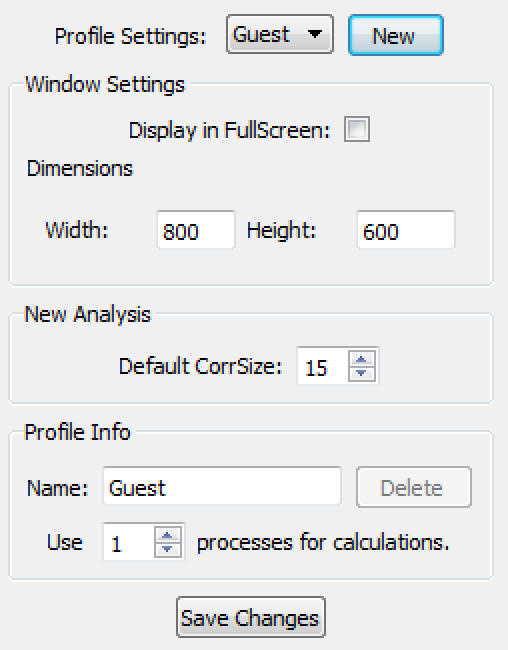
\includegraphics[scale=.6]{profiles}
   \caption{Profile - Define your own preferences}
\end{figure}


  \newpage
  \subsection{Analysis Information}
  \label{sub:Analysis Information}
    \vspace{.2cm}
    \indent\indent Under the \textit{Info} menu, you'll find the analysis information window. This provides you a summary of parameters you've used along with others information regarding your current analysis. One can display data graphs representing different information such as errors encountered during correlation or the current poisson ratio calculated on each image.

\begin{figure}[!h]
   \centering
   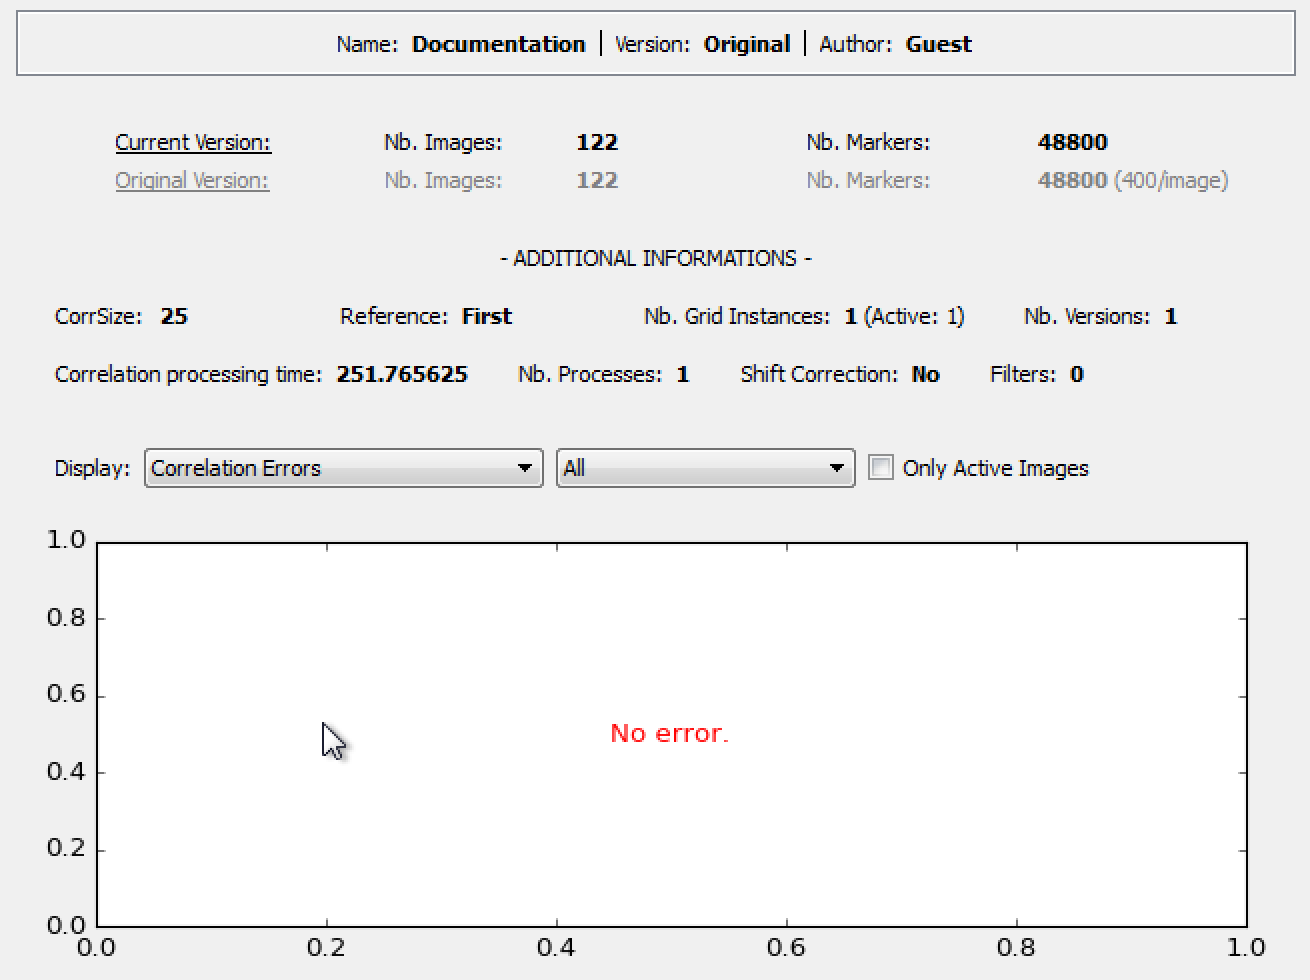
\includegraphics[scale=.4]{analysis_info}
   \caption{Analysis Information : Parameters and more}
\end{figure}


  \subsection{File structure}
  \label{sub:File structure}
    \vspace{.2cm}
    \indent\indent The main information on each correlation process is stored in CSV format. For each analysis, the following files will be created:
\begin{itemize}
  \item \textit{filenamelist.csv} : This file contains names of your images files
  \item \textit{gridx.csv} - \textit{gridy.csv} : These files store respectively the x and y coordinates of each marker in your grids along with their instance number.
  \item \textit{validx.csv} - \textit{validy.csv} : These files store respectively the x and y coordinates of each marker of your analysis. Each line corresponds to a marker, each column corresponds to an image.
  \item \textit{dispx.csv} - \textit{dispy.csv} : These files store respectively the x and y displacements in pixel of each marker of your analysis. Each line corresponds to a marker, each column corresponds to an image.
  \item \textit{stdx.csv} - \textit{stdy.csv} : These files store respectively the x and y standard deviation in pixel of each marker of your analysis. Each line corresponds to a marker, each column corresponds to an image.
  \item \textit{corrcoef.csv} : This file stores the correlation coefficient or each marker of your analysis. Each line correspond to a marker, each column corresponds to an image.
  \item \textit{neighbors.csv} : This file stores the closest neighbors of each marker. Each line correspond to a marker. This file is updated when neighbors are re-calculated.
  \item \textit{infoMarkers.csv} and \textit{infoAnalysis.csv} : These files store informations on your analysis such as correlation errors and parameters used.
  \item \textit{strainx.csv} and \textit{strainy.csv} : These files store the global strain values of each grid along images. Each line corresponds to the image, each column correspond to a grid. These two files are automatically updated when coordinates are re-calculated.
  \item \textit{filter.csv} (Optional) : This file stores information relative to filters applied.
  \item \textit{largeDisp.csv} (Optional) : This file stores the calculated large displacement on your analysis in case the shift correction have been used.
\end{itemize}

\paragraph{Masks\\\newline}
\label{par:Masks}
\newline
\indent Masks (or versions) are saved in the \textit{log} folder of each analysis. This folder is automatically created when the first mask is applied. A mask is then saved whenever markers or images are hide on the analysis. You can always load an old version of your analysis by importing one of these masks.


\end{document}
